\chapter{Agent Based 3D Network on Chip Model}
\label{Chapter.six}

A 3D Network on Chip (NoC) agent based model is a new approach to develop routing algorithms and dynamically monitoring the routing process in a graphical form. In this 3D NoC agent based model, we use a 3D mesh network topology. The model has self directive intelligent agents which are capable of navigating themselves in the network. The architecture of this model will be explained in the following sections. 

\section{Model Architecture}
\vspace{5mm}

The 3D NoC agent based model consists of an Environment and agents such as Packet and RandomAgent. Other elements in the environment include Mesh network, NodeUnit, Node and Path. There are three levels of hierarchy in this model. The levels of hierarchy are represented in Fig.~\ref{fig:6.1}.

\begin{figure}[H]
\vspace{10mm}
\centering
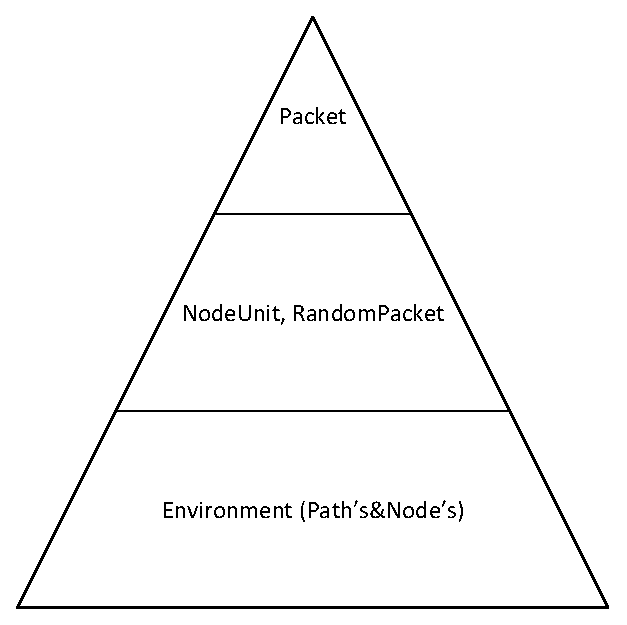
\includegraphics[height=3.0in, width=4.2in]{Level's_of_Heirarchy.eps}
\caption{Levels of hierarchy}
\label{fig:6.1}
\vspace{10mm}
\end{figure} 

In 3D NoC agent based model, Nodes and Paths are collectively called as Environment. It serves as a medium for the other elements in the network to be present. Nodes and Paths belongs to the first level of the hierarchy and are build at the beginning. NodeUnit and RandomAgent are created in the second level of hierarchy. At the final level, packets are created and scheduled. 

\subsection{Environment}
\vspace{5mm}

Environment chosen for this NoC agent based model is 4x4 3D mesh network. Nodes and Paths collectively form an environment. Environment is a  specific region of the window. All the elements and agents of the network should be present within that region. Agents should only move in that designated region. 

\vspace{0.5cm}
\vspace{10mm}
\noindent\textbf{Node}
\vspace{5mm}

\noindent Node is the intersection point of Paths in the network. Node's feature is to keep track of the number of the packets passing by at each time. If the Packet count exceeds certain limit specified by a user, Node class displays a predefined message that there is more traffic at current node location. This information will help a user to develop efficient adaptive routing algorithms.

Nodes are present in a 3-Dimensional (3D) space. Node is a 3D point created at a location $(X,Y,Z)$. A location is of type $Double3D$~\cite{Double3D} which is a predefined class in the MASON class library. 

\vspace{10mm}
\begin{algorithm}[H]
\small % remove to adjust the position and size%
\caption{Creating Nodes in 3-Dimensional space}
\label{alg1}
\begin{boxedminipage}{150mm}
\vspace{5mm}
\begin{algorithmic}[1]
\For{$(x=0;x<=3;x+=1)$}
\For{$(y=0;y<=3;y+=1)$}
\For{$(z=0;z<=3;z+=1)$}        
\State Scale x,y,z coordinates according to the size of the window.
\State Create a node using scaled coordinate values.
\State Schedule the node once all elements of the network are created.
\EndFor
\EndFor
\EndFor
\end{algorithmic}
\vspace{5mm}
\end{boxedminipage}
\end{algorithm}
\vspace{5mm}

Algorithm~\ref{alg1}, is used to create the Nodes in this model. X,Y and Z values are of integer type, since using double values in $for$ loops will lead to complex calculations. In the inner most $for$ loop, scale the X,Y,Z coordinates according to the window size. After the creation of all nodes, they are scheduled.

 
\vspace{0.5cm}
\noindent\textbf{Path}
\vspace{5mm}

\noindent The Path is a line which connects two nodes in the network. A 4x4 3D mesh network is formed with the combination of Paths and Nodes. Nodes are created as explained previously. All created Node objects are stored in a $Bag$. $Bag$ is a predefined class from $sim.util$ package in MASON. $Bag$ maintains a simple array $(objs)$ of objects and the number of objects $(numObjs)$ in the array~\cite{Bag}.

\vspace{0.5cm}
\noindent\textbf{Mesh network}
\vspace{5mm}

To create a 3D 4x4 mesh network, we have used three separate algorithms. These three algorithms are required to create paths along Z-axis, X-axis and Y-axis which form a 3D 4x4 mesh network. The logic for these three algorithms is given below.

\vspace{10mm}
\begin{algorithm}[H]
\small % remove to adjust the position and size%
\caption{Algorithm used to create edges between nodes along the Z-axis}
\label{alg4}
\begin{boxedminipage}{150mm}
\vspace{5mm}
\begin{algorithmic}[1]
\For{$( i=0;i<=62;i++)$}
\Comment{All nodes are stored in a array of type Bag.}
\State $from \gets objs[i]$
\Comment{The node object objs[i] is retried from the bag of nodes.}
\State $to \gets objs[i+1]$
\Comment{The node object objs[i+1] is retried from the bag of nodes.}
\State Draw an edge between $from$ and $to$ nodes.
\Comment{An edge is drawn from objs[i] to objs[i+1].}
\If{$(i>=2)$}
\Comment{Avoid necessary edges to create 3D mesh network} \\
\SWITCH i \\        
 \CASE 2:\CASE 6:\CASE 10:\CASE 14:\CASE 18:\CASE 22:\CASE 26:\CASE 30:\CASE 34:\CASE 38: \CASE 42:\CASE 46:\CASE 50:\CASE 54:\CASE 58: \text{$i++;$} 
 \text{break;} \\
 \CASE Default: \text{break;}
\EndIf
\EndFor
\end{algorithmic}
\vspace{5mm}
\end{boxedminipage}
\end{algorithm}



\vspace{15mm}
\begin{algorithm}[H]
\small % remove to adjust the position and size%
\caption{Algorithm used to create edges along the X-axis}
\label{alg2}
\begin{boxedminipage}{150mm}
\vspace{5mm}
\begin{algorithmic}[1]
\For{$( k=0;k<=47;k++)$}
\State $from \gets objs[k]$
\State $to \gets objs[k+16]$
\State Draw an edge between $from$ and $to$ nodes.
\Comment{An edge is drawn from objs[k] to objs[k+16].}
\EndFor
\end{algorithmic}
\vspace{5mm}
\end{boxedminipage}
\end{algorithm}
\vspace{10mm}

\begin{algorithm}[H]
\small % remove to adjust the position and size%
\caption{Algorithm used to create edges between nodes along the Y-axis}
\label{alg3}
\begin{boxedminipage}{150mm}
\vspace{5mm}
\begin{algorithmic}[1]
\For{$( j=0;j<=59;j++)$}
\State $from \gets objs[j]$
\State $to \gets objs[j+4]$
\State Draw an edge between $from$ and $to$ nodes.
\Comment{An edge is drawn from objs[j] to objs[j+4].}
\If{$(j>=8)$}
\Comment{Avoid unnecessary edges to create 3D mesh network} \\
\SWITCH j \\       
 \CASE 11:\CASE 27:\CASE 43: \text{$j+=4;$} 
 \text{break;} \\
 \CASE Default: \text{break;}
\EndIf
\EndFor
\end{algorithmic}
\vspace{5mm}
\end{boxedminipage}
\end{algorithm}
\vspace{10mm}



After creating the 3D 4x4 mesh network, we need to create all the other elements of the network. Each element is explained in detail below.

\subsection{NodeUnit}
\vspace{5mm}

NodeUnit is one of the main elements of the network. While creating NodeUnits, a user should pass the location coordinates as an argument to method~ \texttt{setNodeUnit}. Then the NodeUnit is created at the specified location. NodeUnit class is responsible for creating and scheduling packets at a particular time. While creating, packets are aware of its destination address to which they need to navigate. Packets direct themselves in the network to reach the specified destination address. Number of packets to be scheduled at NodeUnit is provided by a user in local variable of the NodeUnit class. All the packets scheduled form a single NodeUnit will have same destination location. User can create any number of NodeUnits by using~ \texttt{setNodeUnit} method in class~ \texttt{Noc3D}. 


\subsection{RandomAgent}
\vspace{5mm}

RandomAgent is a random self routing agent. A RandomAgent checks the packets at any random node in the network. RandomAgent's characteristic is to detect any unpredictable packet traffic in the network. 

\vspace{10mm}
\begin{algorithm}[H]
\caption{RandomAgent Logic}
\label{code1}
\begin{boxedminipage}{150mm}
\vspace{5mm}
double[] n = { 0.0, 30.0, 60.0, 90.0};  
\Comment{Array of possible coordinate values.} \\
n[random.nextInt(n.length)];       
\Comment{Choosing a random number from array n.} \\
Choose random numbers for x,y,z coordinates. \\
Set RandomAgent location using these random numbers.
\vspace{5mm}
\end{boxedminipage}
\end{algorithm}
\vspace{10mm}

Whenever RandomAgent encounters a node, it counts the number of packets at that node and displays the packet count, location and current time of the schedule. We stored the possible values for X, Y and Z coordinates in an array. From this array, we retrieved random values to set RandomAgent's position in the network. Logic used for RandomAgent is given in Alg.~\ref{code1}:


\subsection{Packet}
\vspace{5mm}

Packet is designed as a self routing agent in the 3D NoC agent based model. When schedule starts, all the elements of the network are created and then scheduled. Packets are scheduled by NodeUnit at a particular time specified by user. The Packet agent navigates itself in the 3D mesh network. The Packet follows XYZ-routing algorithm to reach the specified destination. In 3D NoC model, each NodeUnit is identified by a location $(X, Y, Z)$. When a Packet arrives to any NodeUnit then the Packet's address $(Cx, Cy, Cz)$ is updated to that of current NodeUnit's address. When creating a Packet, the destination NodeUnit address $(Dx, Dy, Dz)$ is passed as an argument to the object of the Packet class. The Packet is aware of its destination address before the time of scheduling. When the packet is created and scheduled from the NodeUnit, it then follows a XYZ-routing algorithm to reach the destination. The implemented XYZ-routing algorithm in 3D NoC agent based model is shown in Alg.~\ref{alg5}.


In the Alg.~\ref{alg5}, $d$ is the distance between any two nodes in the network. Consider, two nodes as $(x1, y1, z1)$ and $(x2, y2, z2)$. Distance between these two nodes is $d$ which is calculated using the formula $\sqrt{(\Delta X)^2+(\Delta Y)^2+(\Delta Z)^2}$. The formula is expanded as $\sqrt{(x2-x1)^{2}+(y2-y1)^{2}+(z2-z1)^{2}}$. This distance value is required for the Packet to navigate from one node to another. When a Packet is scheduled, in each step the Packet moves and updates its current address to new address. Each time the address is updated either by adding or subtracting the distance value from the appropriate coordinate as per the algorithm. When a Packet reaches the destination then it stops moving and removed from the schedule. 

\vspace{10mm}
\algdef{SE}[IF]{NoThenIf}{EndIf}[1]{\algorithmicif\ #1}{\algorithmicend\ \algorithmicif}
\begin{algorithm}[H]
\small % remove to adjust the position and size%
\caption{XYZ Routing Algorithm}
\label{alg5}
\begin{boxedminipage}{150mm}
\vspace{5mm}
\begin{algorithmic}[1]
\NoThenIf{$(Dx>Cx)$} 
\State Move the Packet to address (Cx+d, Cy, Cz);
\ElsIf{$(Dx<Cx)$} 
\State Move the Packet to address (Cx-d, Cy, Cz);
\ElsIf{$(Dx=Cx)$}
\NoThenIf{$(Dy>Cy)$} 
\State Move the Packet to address (Cx, Cy+d, Cz);
\ElsIf{$(Dy<Cy)$}  
\State Move the Packet to address (Cx, Cy-d, Cz);
\ElsIf{$(Dx=Cx)\&\&(Dy=Cy)$}
\NoThenIf{$(Dz>Cz)$} 
\State Move the Packet to address (Cx, Cy, Cz+d);
\ElsIf{$(Dz<Cz)$}  
\State Move the Packet to address (Cx, Cy, Cz-d);
\Else  
\State Packet reached its destination address (Dx, Dy, Dz);
\EndIf
\EndIf
\EndIf
\end{algorithmic}
\vspace{5mm}
\end{boxedminipage}
\end{algorithm}
\vspace{10mm}

\begin{figure}
\vspace{10mm}
\centering
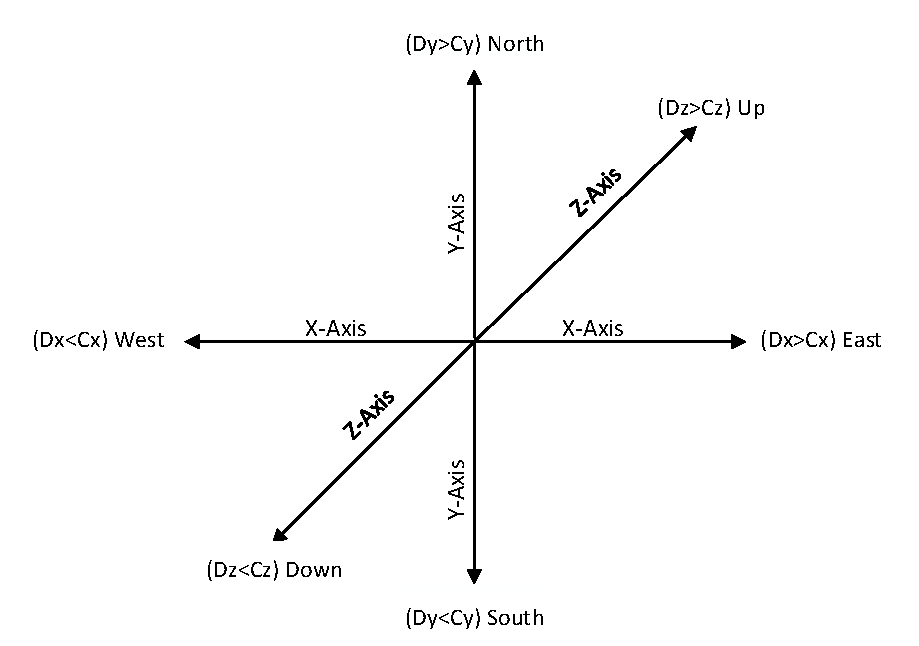
\includegraphics[height=3.0in, width=4.2in]{Directions_with_respect_to_conditional_satements.eps}
\caption{Directions with respect to conditional statements}
\label{fig:6.2}
\vspace{10mm}
\end{figure}

Detailed explanation of the Alg.~\ref{alg5} is as follows: The Current address of Packet is $(Cx, Cy, Cz)$ and destination address is $(Dx, Dy, Dz)$. Firstly, X-coordinate of the current address $(Cx)$ is compared with that of destination address $(Dx)$. Packet moves to East if $Dx>Cx$, West if $Dx<Cx$ and if $Dx=Cx$ it has already aligned in the destination address X-coordinate $(Dx)$. Secondly, $Cy$ is compared with $Dy$. if $Dy>Cy$ the Packet moves to North, if $Dy<Cy$ it moves to South, and if $Dy=Cy$, it has arrived to the corresponding Y-coordinate $(Dy)$. Finally, $Cz$ and $Dz$ are compared with each other. If $Dz>Cz$, then Packet moves up. If $Dz<Cz$, then it moves downwards and if $Dz=Cz$, the packet stops moving further as it has reached its final destination. 

\section{Class Description}
\vspace{5mm}
The package for the 3D NoC agent based model and its classes are explained in detail along with UML representation in this section.

\begin{figure}
\centering
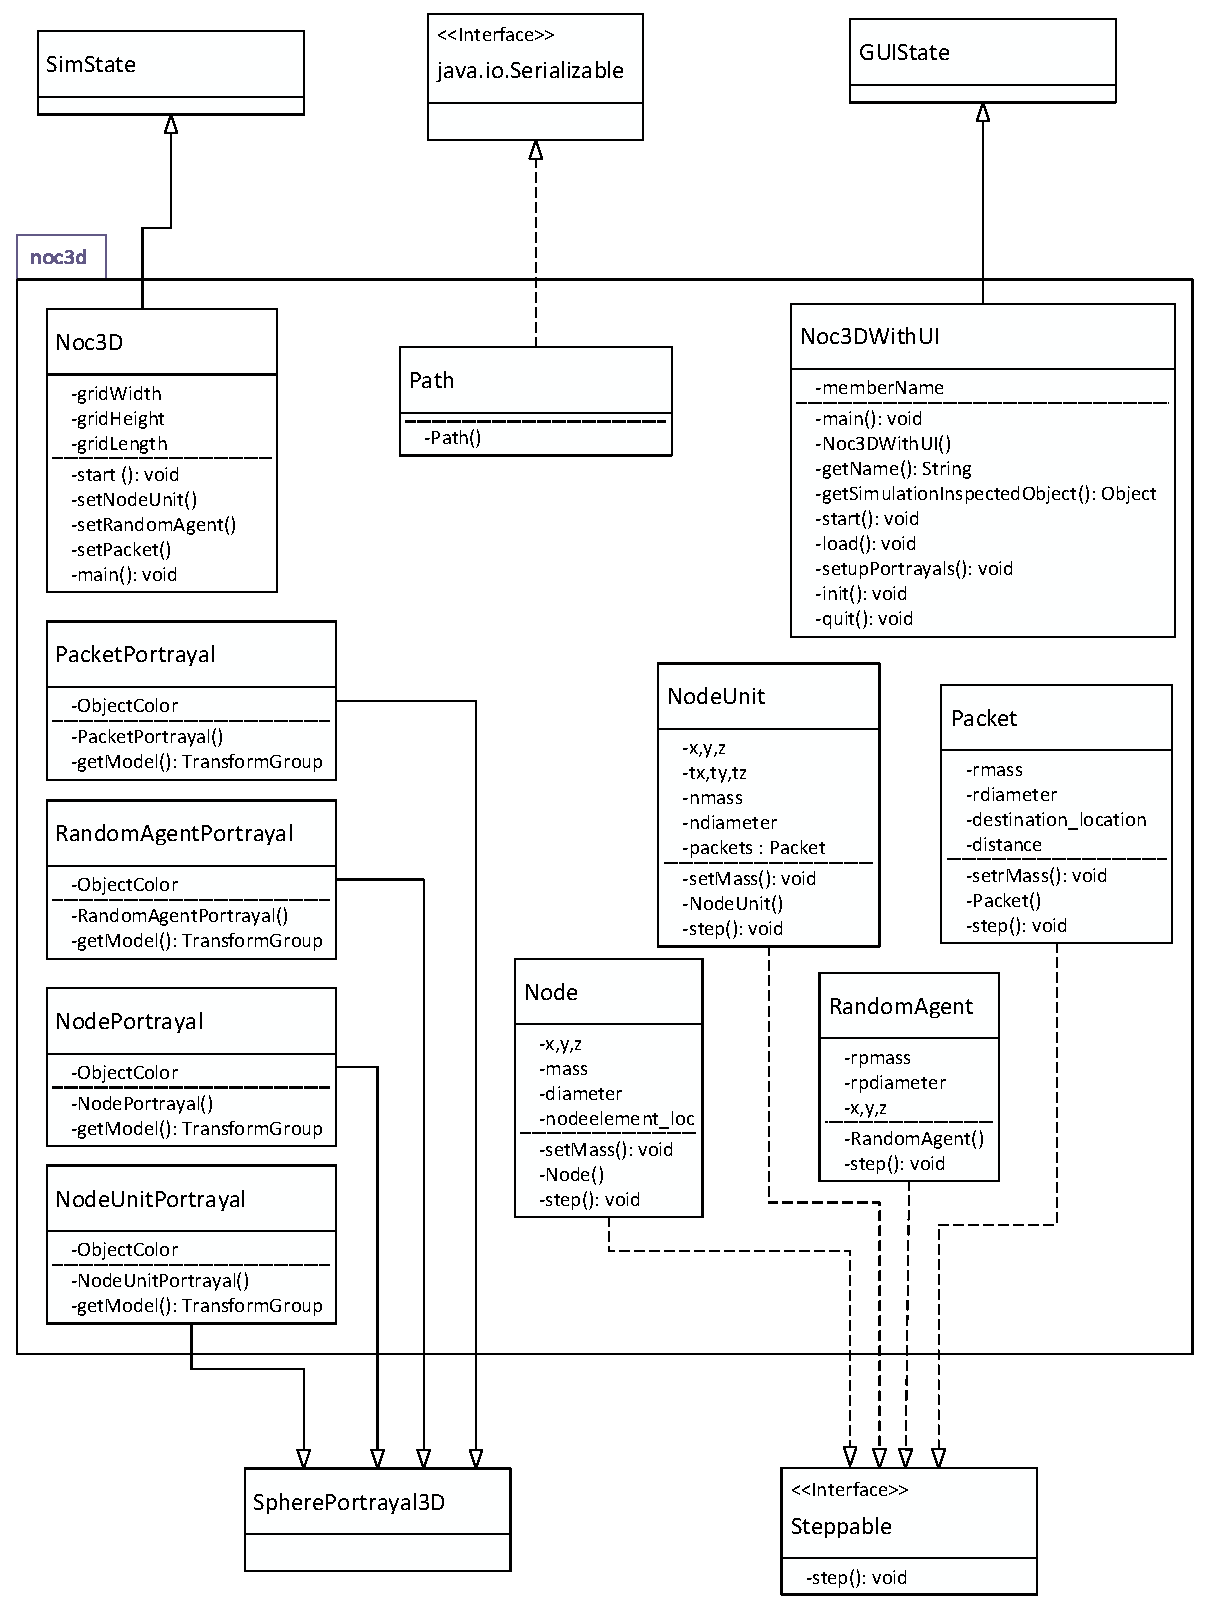
\includegraphics[height=8.4in, width=5.6in]{class_diagram.eps}
\caption{UML class diagram for the 3D NoC agent based model}
\label{fig:6.3}
\end{figure} 

Figure.\ref{fig:6.3} illustrates the group of classes in 3D NoC agent based model. We created all the classes in a single package named ~\texttt{noc3d}. The contents of the noc3d package includes the following classes: \texttt{\seqsplit{NodeUnitPortrayal,~PacketPortrayal,~NodePortrayal,~ RandomAgentPortrayal,~Node,~Packet,~RandomAgent,~Noc3D,~NodeUnit}} and \texttt{~Noc3DWithUI}. These classes are either implemented or inherited from predefined MASON interfaces and classes. Each class has three fields such as the name of the class, parameters and methods in the class. The dotted lines in the diagram represent that the class implements an interface. Solid lines represent the inheritance property of subclass. A subclass is derived from a superclass using extends keyword. Subclass inherits all the protected and public members of the superclass, no matter in which package that subclass is in.

In this model, we have subclasses which are derived from the predefined MASON classes. The~\texttt{Node},~ \texttt{NodeUnit},~ \texttt{RandomAgent} and ~ \texttt{Packet} classes implements the ~\texttt{\seqsplit{Steppable}} ~interface. The~\texttt{Steppable} ~interface allows the elements to perform their respective functionality in each step. The~\texttt{Noc3D} class is inherited from the ~\texttt{SimState} class which helps in scheduling the model. \texttt{\seqsplit{RandomAgentPortrayal,~NodeUnitPortrayal,~PacketPortrayal,~NodePortrayal}} classes implements the ~\texttt{SpherePortrayal3D} interface. This interface influences the physical appearance of elements as a sphere. The \texttt{\seqsplit{Noc3DWithUI}} class is a subclass which is inherited from the superclass ~\texttt{GUIState} which is responsible for visualization. The ~\texttt{Path} ~class implements~ \textit{java.io.serializable} interface. It allows the~ \texttt{Path} ~class to be serializable. 

\section{Schedule}
\vspace{5mm}
3D NoC agent based model is scheduled using MASON multi agent simulation toolkit discussed in Chap.~\ref{Chapter.four}.~ \texttt{SimState} class, from MASON predefined classes, is responsible for the scheduling the model in this toolkit.~ \texttt{Noc3D} class is inherited from~ \texttt{SimState} class.~ \texttt{GUIState} class provides the functionality for visualization.~ \texttt{Noc3DWithUI} class is the subclass which is inherited from superclass~ \texttt{GUIState}. This model can also run without any visualization. User can decide whether he wants to run the model with or without visualization. We can also visualize any of the elements separately using the schedule. For example, it is possible to visualize only nodes without any paths in the schedule. This can be done by choosing the elements which we want to visualize from the list of elements before we start the schedule.

\vspace{15 mm}
\begin{figure}[H] 
\flushleft
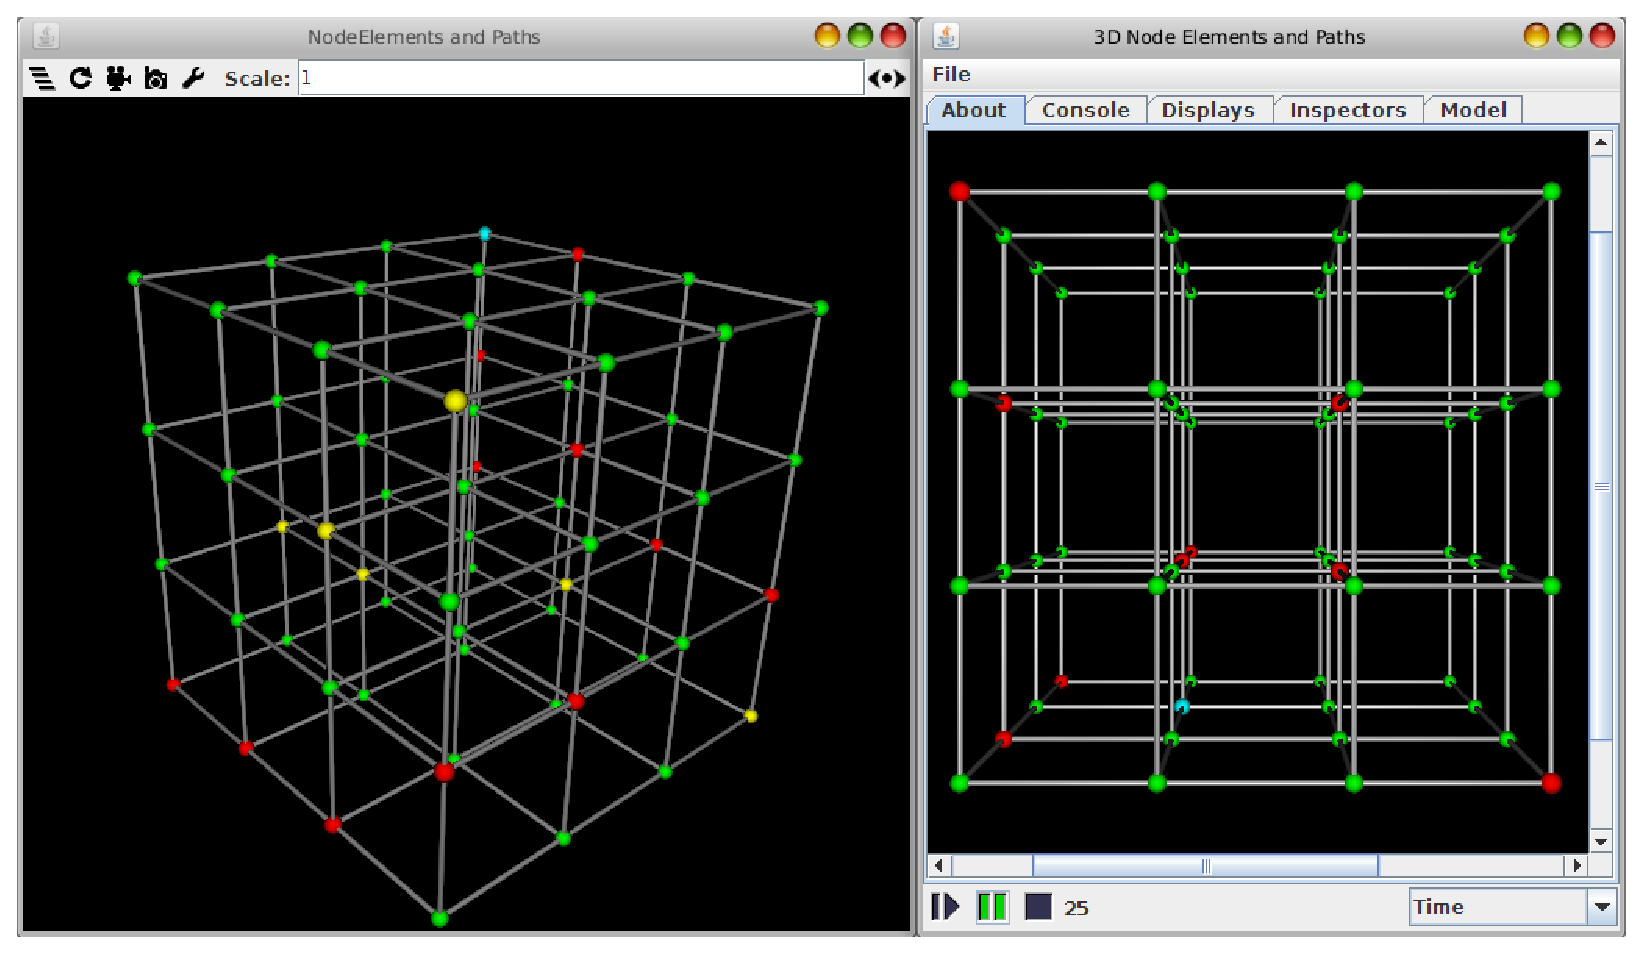
\includegraphics[height=4.4in, width=5.8in]{noc3d.eps}
\caption{Scheduling 3D NoC}
\label{fig:6.4}
\vspace{10mm}
\end{figure} 


As we can see in Fig.\ref{fig:6.4}, two windows will appear when we run the noc3d model either from command-line or with the Eclipse tool. The window on the right side has three buttons, with which one can play, pause and stop the schedule. When we click on play button the schedule starts. It is also possible to start the schedule from certain time by specifying time in the time field before starting the schedule. When schedule begins, the packets and randomagent starts moving from their respective nodes. When all the packets reach their respective destination the packets are removed from the schedule and the schedule ends. In the left window, we can visualize the movement of packets and randomagent in the network. We can also monitor the packets following XYZ-routing algorithm and the number of the packets at each node is displayed at console.  

The yellow spheres are NodeUnit's from where packets are scheduled. Red spheres are packets. Nodes are displayed in green color. Cyan color sphere is a RandomAgent. Paths are in gray color. 
 
\section{Procedure}
\vspace{5mm}

Designing a 3D NoC agent based model with MASON agent based modeling toolkit involves the following steps:

\begin{enumerate}
 \item Download MASON simulation library. Make sure all the dependencies of MASON Java and Java3D are installed in your computer.
 \item Create a package named $noc3d$ in app folder of the MASON tool.Create all the classes in $noc3d$ package.
 \item Create a class ~\texttt{Noc3D}. In ~\texttt{Noc3D} the environment is created using Java3D classes.
 \item Create a node which can keep count of all the packets and gives the count of packets at each instance of time. Include the functionality to identify the packet traffic. When packets count exceeds certain limit a node gives information about when and where the traffic occurred, and the number of the packets present at a node. For this we should access the packet information from environment.
 \item When an agent needs information of other agent, it can be accessed from ~\texttt{Noc3D} class. The access of information is carried out by creating objects to ~\texttt{Noc3D} class.
 \item Implement XYZ- routing algorithm to create self routing packets.
 \item Create a randomagent which visits random nodes in the network and give the count of packets at that node.
 \item Create a class ~\texttt{Noc3DWithUI} which extend the ~\texttt{GUIState} class. This class enables visualization to MASON models.
 \item When we run ~\texttt{Noc3DWithUI}, all the other classes starts their schedule and runs until $``exit''$ command is encountered.
 \item Run model using command $``java~sim.app.noc3d.Noc3DWithUI''$.
\end{enumerate}








